 \documentclass{article}
\usepackage[utf8]{inputenc}
\usepackage[a4paper, total={7in, 10in}]{geometry}
\usepackage{braket}
\usepackage{xcolor}
\usepackage{amsmath}
\usepackage{amssymb}
\usepackage{amsfonts}
\usepackage{graphicx}
\usepackage{svg}
\usepackage{float}
\usepackage{tikz}
\usepackage[ruled,vlined]{algorithm2e}
\usepackage{multicol}
\usepackage[backend=biber,style=alphabetic,sorting=ynt]{biblatex}
\usepackage{xcolor}
%\addbibresource{sample.bib} %Import the bibliography file

\newcommand{\commentt}[1]{\textcolor{blue}{ \textbf{[COMMENT]} #1}}
\newcommand{\ctt}[1]{\commentt{#1}}
\newcommand{\prb}[1]{ \mathbf{Pr} \left[ {#1} \right]}
\newcommand{\onotation}[1]{\(\mathcal{O} \left( {#1}  \right) \)}
\newcommand{\ona}[1]{\onotation{#1}}
\newcommand{\PSI}{{\ket{\psi}}}
\newcommand{\LESn}{\ket{\psi_n}}
\newcommand{\LESa}{\ket{\phi_n}}
\newcommand{\LESs}{\frac{1}{\sqrt{n}}\sum_{i}{\ket{\left(0^{i}10^{n-i}\right)^{n}}}}
\newcommand{\Hn}{\mathcal{H}_{n}}
\newcommand{\Ep}{\frac{1}{\sqrt{2^n}}\sum^{2^n}_{x}{ \ket{xx}}}
\newcommand{\HON}{\ket{\psi_{\text{honest}}}}
\newcommand{\Lemma}{\paragraph{Lemma.}}


\setlength{\columnsep}{0.6cm}

\newcommand{\Gz}{ G_{z}^{\delta} } 

\begin{document}

\title{Quantum LTC With Positive Rate}
\author{David Ponarovsky}
\maketitle
%\begin{multicols*}{2}
\newcommand{ \Hw }{ \delta\Delta -\Delta^{\frac{1}{2}-\varepsilon}/\delta  }
	\newcommand{ \Nw }{ \Delta^{\frac{3}{2}-\varepsilon}} 
	  \newcommand{ \Gu } { \Gamma^{\cup} }
	  \newcommand{ \Guq } { \Gamma^{\cup, \square} }

    	\newcommand{ \Gsa } {\Gamma_{\square_{1}} }
	\newcommand{ \Gsb } {\Gamma_{\square_{2}} }
        \newcommand{ \Aa } { C_{A_{1}}}  
	\newcommand{ \Ab } { C_{A_{2}}}
	\newcommand{ \Ac } { C_{A_{3}}}
	\newcommand{ \Aab } { \Aa \otimes \Ab } 
	\newcommand{ \Aac } { \Aa \otimes \Ac }
	\newcommand{ \Aabc } { \Aa \otimes \Ab \otimes \Ac }
	\newcommand{ \Aabp } { \Aa^{\perp} \otimes \Ab^{\perp} } 
	\newcommand{ \Aacp } { \Aa^{\perp} \otimes \Ac^{\perp} }
	\newcommand{ \Aabcp } { \Aa^{\perp} \otimes \Ab^{\perp} \otimes \Ac^{\perp} }
	\newcommand{ \Aabpp } { \left( \Aabp \right)^\perp } 
	\newcommand{ \Aacpp } { \left( \Aacp \right)^\perp }
	\newcommand{ \Aabcpp } { \left( \Aabcp \right)^\perp }
	\newcommand{ \YY } {  y_{1}y_{2}^{\top} }
	\newcommand{ \ZZ } {  z_{1}z_{2}^{\top} } 
	\newcommand{ \TT } { \tilde{\tau} } 


  \paragraph{preamble.} preamble.  
  \begin{figure}[H]
            %\label{fig:square}
            \begin{center}
            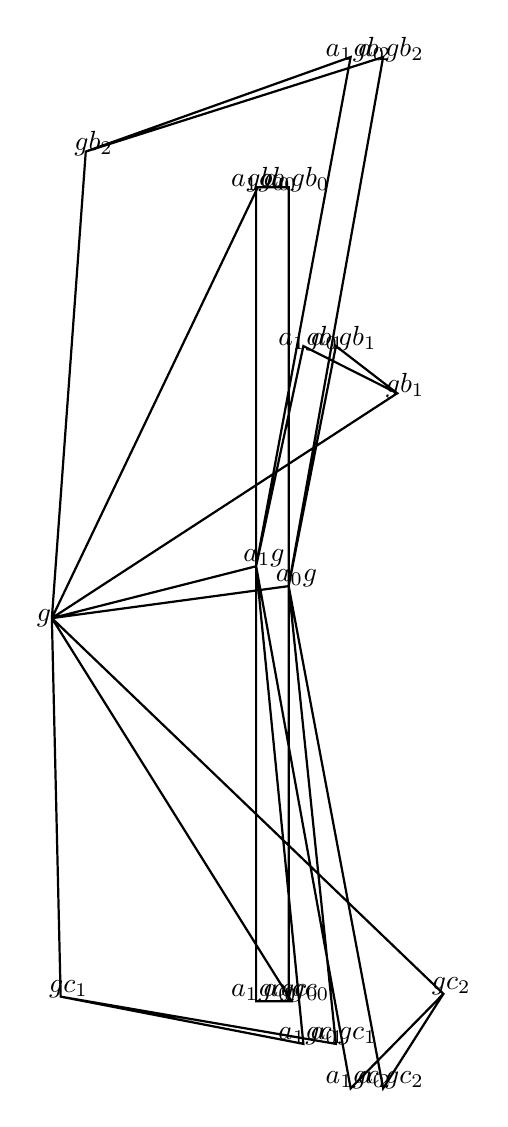
\begin{tikzpicture}
            \draw[thick](0,0)(0,0) -- (2.6160236609006846,5.472111986589232) -- (3.007192885963593,5.472111986589232) -- (3.007192885963593,0.4064777918768201) -- (0,0)
(0,0) -- (4.385697009732788,2.855274502899741) -- (3.607192885963593,3.455274502899741) -- (3.007192885963593,0.4064777918768201) -- (0,0)
(0,0) -- (0.43061841995968797,5.925382368824403) -- (4.207192885963593,7.125382368824403) -- (3.007192885963593,0.4064777918768201) -- (0,0)
(0,0) -- (2.6160236609006846,5.472111986589232) -- (2.5941079965374056,5.472111986589232) -- (2.5941079965374056,0.6588561111857653) -- (0,0)
(0,0) -- (4.385697009732788,2.855274502899741) -- (3.1941079965374057,3.455274502899741) -- (2.5941079965374056,0.6588561111857653) -- (0,0)
(0,0) -- (0.43061841995968797,5.925382368824403) -- (3.794107996537406,7.125382368824403) -- (2.5941079965374056,0.6588561111857653) -- (0,0)
(0,0) -- (3.043465718432985,-4.865545814811391) -- (3.007192885963593,-4.865545814811391) -- (3.007192885963593,0.4064777918768201) -- (0,0)
(0,0) -- (0.11163741729040833,-4.807092204172177) -- (3.607192885963593,-5.4070922041721765) -- (3.007192885963593,0.4064777918768201) -- (0,0)
(0,0) -- (4.972148712687328,-4.771657399261202) -- (4.207192885963593,-5.971657399261202) -- (3.007192885963593,0.4064777918768201) -- (0,0)
(0,0) -- (3.043465718432985,-4.865545814811391) -- (2.5941079965374056,-4.865545814811391) -- (2.5941079965374056,0.6588561111857653) -- (0,0)
(0,0) -- (0.11163741729040833,-4.807092204172177) -- (3.1941079965374057,-5.4070922041721765) -- (2.5941079965374056,0.6588561111857653) -- (0,0)
(0,0) -- (4.972148712687328,-4.771657399261202) -- (3.794107996537406,-5.971657399261202) -- (2.5941079965374056,0.6588561111857653) -- (0,0)
;
\node at (3.107192885963593,5.572111986589231) {$ a_{ 0  } gb_{ 0 } $};
\node at (3.707192885963593,3.5552745028997412) {$ a_{ 0  } gb_{ 1 } $};
\node at (4.307192885963593,7.225382368824403) {$ a_{ 0  } gb_{ 2 } $};
\node at (2.6941079965374057,5.572111986589231) {$ a_{ 1  } gb_{ 0 } $};
\node at (3.294107996537406,3.5552745028997412) {$ a_{ 1  } gb_{ 1 } $};
\node at (3.894107996537406,7.225382368824403) {$ a_{ 1  } gb_{ 2 } $};
\node at (3.107192885963593,-4.765545814811391) {$ a_{ 0  } gc_{ 0 } $};
\node at (3.707192885963593,-5.307092204172177) {$ a_{ 0  } gc_{ 1 } $};
\node at (4.307192885963593,-5.871657399261203) {$ a_{ 0  } gc_{ 2 } $};
\node at (2.6941079965374057,-4.765545814811391) {$ a_{ 1  } gc_{ 0 } $};
\node at (3.294107996537406,-5.307092204172177) {$ a_{ 1  } gc_{ 1 } $};
\node at (3.894107996537406,-5.871657399261203) {$ a_{ 1  } gc_{ 2 } $};
\node at (-0.1,0) {$ g $};
\node at (3.107192885963593,0.5064777918768201) {$ a_{ 0 }g $};
\node at (2.6941079965374057,0.7588561111857652) {$ a_{ 1 }g $};
\node at (2.7160236609006847,5.572111986589231) {$ gb_{ 0 } $};
\node at (4.485697009732788,2.955274502899741) {$ gb_{ 1 } $};
\node at (0.530618419959688,6.025382368824403) {$ gb_{ 2 } $};
\node at (3.143465718432985,-4.765545814811391) {$ gc_{ 0 } $};
\node at (0.21163741729040833,-4.707092204172177) {$ gc_{ 1 } $};
\node at (5.072148712687327,-4.6716573992612025) {$ gc_{ 2 } $};

            \end{tikzpicture}
            \end{center}
            \caption{Square of the complex, with edges $(g,ag), (agb, gb) \in E_A,
            (g,gb), (agb, ag) \in E_B.$ \label{fig:square}
            }
            \end{figure}
 \begin{figure}[H]
            %\label{fig:square}
            \begin{center}
            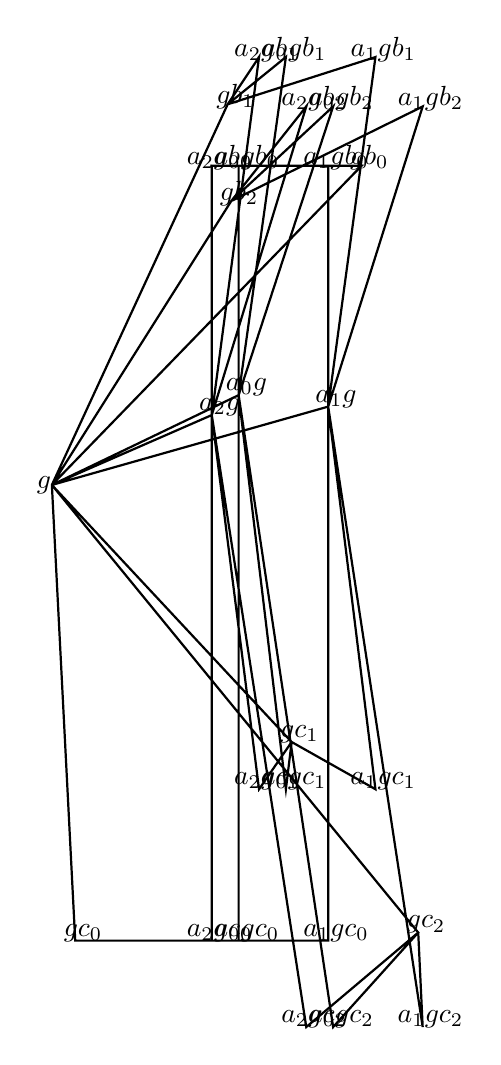
\begin{tikzpicture}
            \draw[thick](0,0)(0,0) -- (3.93233616919947,4.053180613650017) -- (2.371962443224904,4.053180613650017) -- (2.371962443224904,1.140709063538863) -- (0,0)
(0,0) -- (2.2326106404964934,4.834095674457727) -- (2.971962443224904,5.434095674457726) -- (2.371962443224904,1.140709063538863) -- (0,0)
(0,0) -- (2.278617338883083,3.6063663038890743) -- (3.571962443224904,4.8063663038890745) -- (2.371962443224904,1.140709063538863) -- (0,0)
(0,0) -- (3.93233616919947,4.053180613650017) -- (3.5092953531321234,4.053180613650017) -- (3.5092953531321234,0.9948861190823967) -- (0,0)
(0,0) -- (2.2326106404964934,4.834095674457727) -- (4.109295353132123,5.434095674457726) -- (3.5092953531321234,0.9948861190823967) -- (0,0)
(0,0) -- (2.278617338883083,3.6063663038890743) -- (4.7092953531321236,4.8063663038890745) -- (3.5092953531321234,0.9948861190823967) -- (0,0)
(0,0) -- (3.93233616919947,4.053180613650017) -- (2.0309528848636575,4.053180613650017) -- (2.0309528848636575,0.8875379570569631) -- (0,0)
(0,0) -- (2.2326106404964934,4.834095674457727) -- (2.6309528848636576,5.434095674457726) -- (2.0309528848636575,0.8875379570569631) -- (0,0)
(0,0) -- (2.278617338883083,3.6063663038890743) -- (3.2309528848636573,4.8063663038890745) -- (2.0309528848636575,0.8875379570569631) -- (0,0)
(0,0) -- (0.29654872876081373,-5.787031870239331) -- (2.371962443224904,-5.787031870239331) -- (2.371962443224904,1.140709063538863) -- (0,0)
(0,0) -- (3.0449446097400323,-3.2642206298845875) -- (2.971962443224904,-3.8642206298845876) -- (2.371962443224904,1.140709063538863) -- (0,0)
(0,0) -- (4.6527158746740955,-5.684405893917516) -- (3.571962443224904,-6.884405893917516) -- (2.371962443224904,1.140709063538863) -- (0,0)
(0,0) -- (0.29654872876081373,-5.787031870239331) -- (3.5092953531321234,-5.787031870239331) -- (3.5092953531321234,0.9948861190823967) -- (0,0)
(0,0) -- (3.0449446097400323,-3.2642206298845875) -- (4.109295353132123,-3.8642206298845876) -- (3.5092953531321234,0.9948861190823967) -- (0,0)
(0,0) -- (4.6527158746740955,-5.684405893917516) -- (4.7092953531321236,-6.884405893917516) -- (3.5092953531321234,0.9948861190823967) -- (0,0)
(0,0) -- (0.29654872876081373,-5.787031870239331) -- (2.0309528848636575,-5.787031870239331) -- (2.0309528848636575,0.8875379570569631) -- (0,0)
(0,0) -- (3.0449446097400323,-3.2642206298845875) -- (2.6309528848636576,-3.8642206298845876) -- (2.0309528848636575,0.8875379570569631) -- (0,0)
(0,0) -- (4.6527158746740955,-5.684405893917516) -- (3.2309528848636573,-6.884405893917516) -- (2.0309528848636575,0.8875379570569631) -- (0,0)
;
\node at (2.471962443224904,4.153180613650017) {$ a_{ 0  } gb_{ 0 } $};
\node at (3.071962443224904,5.534095674457726) {$ a_{ 0  } gb_{ 1 } $};
\node at (3.671962443224904,4.906366303889074) {$ a_{ 0  } gb_{ 2 } $};
\node at (3.6092953531321235,4.153180613650017) {$ a_{ 1  } gb_{ 0 } $};
\node at (4.209295353132123,5.534095674457726) {$ a_{ 1  } gb_{ 1 } $};
\node at (4.809295353132123,4.906366303889074) {$ a_{ 1  } gb_{ 2 } $};
\node at (2.1309528848636576,4.153180613650017) {$ a_{ 2  } gb_{ 0 } $};
\node at (2.7309528848636577,5.534095674457726) {$ a_{ 2  } gb_{ 1 } $};
\node at (3.3309528848636574,4.906366303889074) {$ a_{ 2  } gb_{ 2 } $};
\node at (2.471962443224904,-5.687031870239331) {$ a_{ 0  } gc_{ 0 } $};
\node at (3.071962443224904,-3.7642206298845875) {$ a_{ 0  } gc_{ 1 } $};
\node at (3.671962443224904,-6.7844058939175165) {$ a_{ 0  } gc_{ 2 } $};
\node at (3.6092953531321235,-5.687031870239331) {$ a_{ 1  } gc_{ 0 } $};
\node at (4.209295353132123,-3.7642206298845875) {$ a_{ 1  } gc_{ 1 } $};
\node at (4.809295353132123,-6.7844058939175165) {$ a_{ 1  } gc_{ 2 } $};
\node at (2.1309528848636576,-5.687031870239331) {$ a_{ 2  } gc_{ 0 } $};
\node at (2.7309528848636577,-3.7642206298845875) {$ a_{ 2  } gc_{ 1 } $};
\node at (3.3309528848636574,-6.7844058939175165) {$ a_{ 2  } gc_{ 2 } $};
\node at (-0.1,0) {$ g $};
\node at (2.471962443224904,1.2407090635388631) {$ a_{ 0 }g $};
\node at (3.6092953531321235,1.0948861190823966) {$ a_{ 1 }g $};
\node at (2.1309528848636576,0.9875379570569631) {$ a_{ 2 }g $};
\node at (4.0323361691994695,4.153180613650017) {$ gb_{ 0 } $};
\node at (2.3326106404964935,4.934095674457726) {$ gb_{ 1 } $};
\node at (2.378617338883083,3.7063663038890744) {$ gb_{ 2 } $};
\node at (0.3965487287608137,-5.687031870239331) {$ gc_{ 0 } $};
\node at (3.1449446097400324,-3.1642206298845874) {$ gc_{ 1 } $};
\node at (4.752715874674095,-5.584405893917516) {$ gc_{ 2 } $};

            \end{tikzpicture}
            \end{center}
            \caption{Square of the complex, with edges $(g,ag), (agb, gb) \in E_A,
            (g,gb), (agb, ag) \in E_B.$ \label{fig:square}
            }
            \end{figure}
 \begin{figure}[H]
            %\label{fig:square}
            \begin{center}
            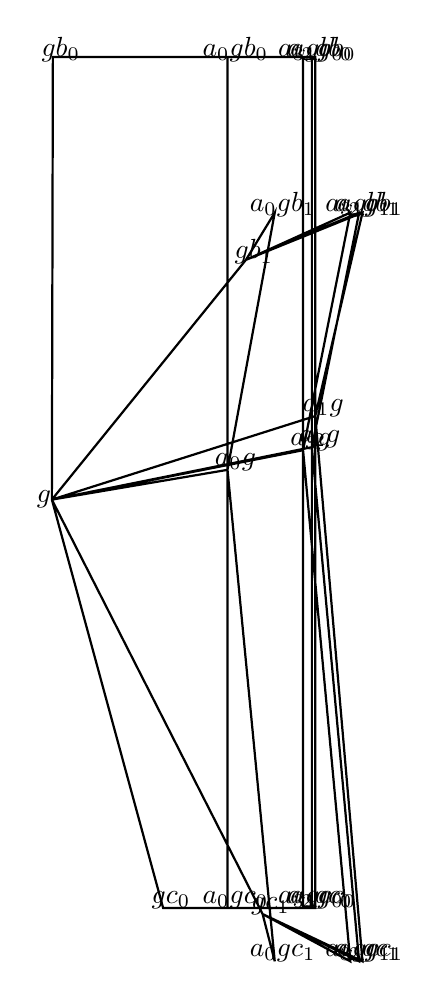
\begin{tikzpicture}
            \draw[thick](0,0)(0,0) -- (0.012727275013436623,5.620424619445986) -- (2.2305928019112296,5.620424619445986) -- (2.2305928019112296,0.37814911895979236) -- (0,0)
(0,0) -- (2.4647723995844135,3.044902336754086) -- (2.8305928019112296,3.644902336754086) -- (2.2305928019112296,0.37814911895979236) -- (0,0)
(0,0) -- (0.012727275013436623,5.620424619445986) -- (3.345048422018217,5.620424619445986) -- (3.345048422018217,1.0615199391544679) -- (0,0)
(0,0) -- (2.4647723995844135,3.044902336754086) -- (3.945048422018217,3.644902336754086) -- (3.345048422018217,1.0615199391544679) -- (0,0)
(0,0) -- (0.012727275013436623,5.620424619445986) -- (3.3019767367308948,5.620424619445986) -- (3.3019767367308948,0.6661529659081382) -- (0,0)
(0,0) -- (2.4647723995844135,3.044902336754086) -- (3.901976736730895,3.644902336754086) -- (3.3019767367308948,0.6661529659081382) -- (0,0)
(0,0) -- (0.012727275013436623,5.620424619445986) -- (3.1901385740739787,5.620424619445986) -- (3.1901385740739787,0.6275645227987656) -- (0,0)
(0,0) -- (2.4647723995844135,3.044902336754086) -- (3.790138574073979,3.644902336754086) -- (3.1901385740739787,0.6275645227987656) -- (0,0)
(0,0) -- (1.413021316746882,-5.1865808056600065) -- (2.2305928019112296,-5.1865808056600065) -- (2.2305928019112296,0.37814911895979236) -- (0,0)
(0,0) -- (2.6763851133520804,-5.2633054554025716) -- (2.8305928019112296,-5.863305455402571) -- (2.2305928019112296,0.37814911895979236) -- (0,0)
(0,0) -- (1.413021316746882,-5.1865808056600065) -- (3.345048422018217,-5.1865808056600065) -- (3.345048422018217,1.0615199391544679) -- (0,0)
(0,0) -- (2.6763851133520804,-5.2633054554025716) -- (3.945048422018217,-5.863305455402571) -- (3.345048422018217,1.0615199391544679) -- (0,0)
(0,0) -- (1.413021316746882,-5.1865808056600065) -- (3.3019767367308948,-5.1865808056600065) -- (3.3019767367308948,0.6661529659081382) -- (0,0)
(0,0) -- (2.6763851133520804,-5.2633054554025716) -- (3.901976736730895,-5.863305455402571) -- (3.3019767367308948,0.6661529659081382) -- (0,0)
(0,0) -- (1.413021316746882,-5.1865808056600065) -- (3.1901385740739787,-5.1865808056600065) -- (3.1901385740739787,0.6275645227987656) -- (0,0)
(0,0) -- (2.6763851133520804,-5.2633054554025716) -- (3.790138574073979,-5.863305455402571) -- (3.1901385740739787,0.6275645227987656) -- (0,0)
;
\node at (2.3305928019112296,5.720424619445986) {$ a_{ 0  } gb_{ 0 } $};
\node at (2.9305928019112297,3.744902336754086) {$ a_{ 0  } gb_{ 1 } $};
\node at (3.445048422018217,5.720424619445986) {$ a_{ 1  } gb_{ 0 } $};
\node at (4.045048422018217,3.744902336754086) {$ a_{ 1  } gb_{ 1 } $};
\node at (3.401976736730895,5.720424619445986) {$ a_{ 2  } gb_{ 0 } $};
\node at (4.001976736730895,3.744902336754086) {$ a_{ 2  } gb_{ 1 } $};
\node at (3.290138574073979,5.720424619445986) {$ a_{ 3  } gb_{ 0 } $};
\node at (3.890138574073979,3.744902336754086) {$ a_{ 3  } gb_{ 1 } $};
\node at (2.3305928019112296,-5.086580805660007) {$ a_{ 0  } gc_{ 0 } $};
\node at (2.9305928019112297,-5.7633054554025716) {$ a_{ 0  } gc_{ 1 } $};
\node at (3.445048422018217,-5.086580805660007) {$ a_{ 1  } gc_{ 0 } $};
\node at (4.045048422018217,-5.7633054554025716) {$ a_{ 1  } gc_{ 1 } $};
\node at (3.401976736730895,-5.086580805660007) {$ a_{ 2  } gc_{ 0 } $};
\node at (4.001976736730895,-5.7633054554025716) {$ a_{ 2  } gc_{ 1 } $};
\node at (3.290138574073979,-5.086580805660007) {$ a_{ 3  } gc_{ 0 } $};
\node at (3.890138574073979,-5.7633054554025716) {$ a_{ 3  } gc_{ 1 } $};
\node at (-0.1,0) {$ g $};
\node at (2.3305928019112296,0.4781491189597924) {$ a_{ 0 }g $};
\node at (3.445048422018217,1.161519939154468) {$ a_{ 1 }g $};
\node at (3.401976736730895,0.7661529659081382) {$ a_{ 2 }g $};
\node at (3.290138574073979,0.7275645227987656) {$ a_{ 3 }g $};
\node at (0.11272727501343663,5.720424619445986) {$ gb_{ 0 } $};
\node at (2.5647723995844136,3.144902336754086) {$ gb_{ 1 } $};
\node at (1.513021316746882,-5.086580805660007) {$ gc_{ 0 } $};
\node at (2.7763851133520805,-5.163305455402572) {$ gc_{ 1 } $};

            \end{tikzpicture}
            \end{center}
            \caption{Square of the complex, with edges $(g,ag), (agb, gb) \in E_A,
            (g,gb), (agb, ag) \in E_B.$ \label{fig:square}
            }
            \end{figure}
 \begin{figure}[H]
            %\label{fig:square}
            \begin{center}
            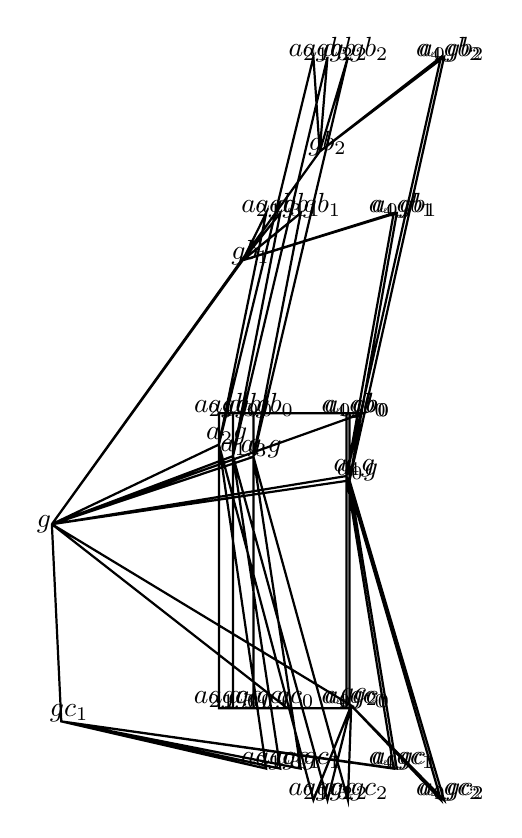
\begin{tikzpicture}
            \draw[thick](0,0)(0,0) -- (3.9501052793929388,1.4091744323219415) -- (3.780353993183975,1.4091744323219415) -- (3.780353993183975,0.5553988183641999) -- (0,0)
(0,0) -- (2.423237708216531,3.3513026855293346) -- (4.380353993183975,3.9513026855293347) -- (3.780353993183975,0.5553988183641999) -- (0,0)
(0,0) -- (3.401369820287759,4.732329732746871) -- (4.980353993183975,5.932329732746871) -- (3.780353993183975,0.5553988183641999) -- (0,0)
(0,0) -- (3.9501052793929388,1.4091744323219415) -- (2.3004174520927956,1.4091744323219415) -- (2.3004174520927956,0.8651026981976262) -- (0,0)
(0,0) -- (2.423237708216531,3.3513026855293346) -- (2.9004174520927957,3.9513026855293347) -- (2.3004174520927956,0.8651026981976262) -- (0,0)
(0,0) -- (3.401369820287759,4.732329732746871) -- (3.5004174520927958,5.932329732746871) -- (2.3004174520927956,0.8651026981976262) -- (0,0)
(0,0) -- (3.9501052793929388,1.4091744323219415) -- (2.12172869247346,1.4091744323219415) -- (2.12172869247346,1.0119049388509627) -- (0,0)
(0,0) -- (2.423237708216531,3.3513026855293346) -- (2.72172869247346,3.9513026855293347) -- (2.12172869247346,1.0119049388509627) -- (0,0)
(0,0) -- (3.401369820287759,4.732329732746871) -- (3.32172869247346,5.932329732746871) -- (2.12172869247346,1.0119049388509627) -- (0,0)
(0,0) -- (3.9501052793929388,1.4091744323219415) -- (2.5598460711193844,1.4091744323219415) -- (2.5598460711193844,0.8556891726299559) -- (0,0)
(0,0) -- (2.423237708216531,3.3513026855293346) -- (3.1598460711193845,3.9513026855293347) -- (2.5598460711193844,0.8556891726299559) -- (0,0)
(0,0) -- (3.401369820287759,4.732329732746871) -- (3.7598460711193846,5.932329732746871) -- (2.5598460711193844,0.8556891726299559) -- (0,0)
(0,0) -- (3.9501052793929388,1.4091744323219415) -- (3.741495596790804,1.4091744323219415) -- (3.741495596790804,0.6115585609446708) -- (0,0)
(0,0) -- (2.423237708216531,3.3513026855293346) -- (4.3414955967908035,3.9513026855293347) -- (3.741495596790804,0.6115585609446708) -- (0,0)
(0,0) -- (3.401369820287759,4.732329732746871) -- (4.941495596790804,5.932329732746871) -- (3.741495596790804,0.6115585609446708) -- (0,0)
(0,0) -- (2.9914049700770247,-2.337957360451259) -- (3.780353993183975,-2.337957360451259) -- (3.780353993183975,0.5553988183641999) -- (0,0)
(0,0) -- (0.11962480839246503,-2.5044716616782674) -- (4.380353993183975,-3.1044716616782675) -- (3.780353993183975,0.5553988183641999) -- (0,0)
(0,0) -- (3.8018662132167487,-2.3029773150782087) -- (4.980353993183975,-3.5029773150782084) -- (3.780353993183975,0.5553988183641999) -- (0,0)
(0,0) -- (2.9914049700770247,-2.337957360451259) -- (2.3004174520927956,-2.337957360451259) -- (2.3004174520927956,0.8651026981976262) -- (0,0)
(0,0) -- (0.11962480839246503,-2.5044716616782674) -- (2.9004174520927957,-3.1044716616782675) -- (2.3004174520927956,0.8651026981976262) -- (0,0)
(0,0) -- (3.8018662132167487,-2.3029773150782087) -- (3.5004174520927958,-3.5029773150782084) -- (2.3004174520927956,0.8651026981976262) -- (0,0)
(0,0) -- (2.9914049700770247,-2.337957360451259) -- (2.12172869247346,-2.337957360451259) -- (2.12172869247346,1.0119049388509627) -- (0,0)
(0,0) -- (0.11962480839246503,-2.5044716616782674) -- (2.72172869247346,-3.1044716616782675) -- (2.12172869247346,1.0119049388509627) -- (0,0)
(0,0) -- (3.8018662132167487,-2.3029773150782087) -- (3.32172869247346,-3.5029773150782084) -- (2.12172869247346,1.0119049388509627) -- (0,0)
(0,0) -- (2.9914049700770247,-2.337957360451259) -- (2.5598460711193844,-2.337957360451259) -- (2.5598460711193844,0.8556891726299559) -- (0,0)
(0,0) -- (0.11962480839246503,-2.5044716616782674) -- (3.1598460711193845,-3.1044716616782675) -- (2.5598460711193844,0.8556891726299559) -- (0,0)
(0,0) -- (3.8018662132167487,-2.3029773150782087) -- (3.7598460711193846,-3.5029773150782084) -- (2.5598460711193844,0.8556891726299559) -- (0,0)
(0,0) -- (2.9914049700770247,-2.337957360451259) -- (3.741495596790804,-2.337957360451259) -- (3.741495596790804,0.6115585609446708) -- (0,0)
(0,0) -- (0.11962480839246503,-2.5044716616782674) -- (4.3414955967908035,-3.1044716616782675) -- (3.741495596790804,0.6115585609446708) -- (0,0)
(0,0) -- (3.8018662132167487,-2.3029773150782087) -- (4.941495596790804,-3.5029773150782084) -- (3.741495596790804,0.6115585609446708) -- (0,0)
;
\node at (3.880353993183975,1.5091744323219416) {$ a_{ 0  } gb_{ 0 } $};
\node at (4.480353993183974,4.051302685529334) {$ a_{ 0  } gb_{ 1 } $};
\node at (5.080353993183975,6.032329732746871) {$ a_{ 0  } gb_{ 2 } $};
\node at (2.4004174520927957,1.5091744323219416) {$ a_{ 1  } gb_{ 0 } $};
\node at (3.0004174520927958,4.051302685529334) {$ a_{ 1  } gb_{ 1 } $};
\node at (3.600417452092796,6.032329732746871) {$ a_{ 1  } gb_{ 2 } $};
\node at (2.22172869247346,1.5091744323219416) {$ a_{ 2  } gb_{ 0 } $};
\node at (2.82172869247346,4.051302685529334) {$ a_{ 2  } gb_{ 1 } $};
\node at (3.4217286924734602,6.032329732746871) {$ a_{ 2  } gb_{ 2 } $};
\node at (2.6598460711193845,1.5091744323219416) {$ a_{ 3  } gb_{ 0 } $};
\node at (3.2598460711193846,4.051302685529334) {$ a_{ 3  } gb_{ 1 } $};
\node at (3.8598460711193847,6.032329732746871) {$ a_{ 3  } gb_{ 2 } $};
\node at (3.841495596790804,1.5091744323219416) {$ a_{ 4  } gb_{ 0 } $};
\node at (4.441495596790803,4.051302685529334) {$ a_{ 4  } gb_{ 1 } $};
\node at (5.041495596790804,6.032329732746871) {$ a_{ 4  } gb_{ 2 } $};
\node at (3.880353993183975,-2.237957360451259) {$ a_{ 0  } gc_{ 0 } $};
\node at (4.480353993183974,-3.0044716616782674) {$ a_{ 0  } gc_{ 1 } $};
\node at (5.080353993183975,-3.4029773150782083) {$ a_{ 0  } gc_{ 2 } $};
\node at (2.4004174520927957,-2.237957360451259) {$ a_{ 1  } gc_{ 0 } $};
\node at (3.0004174520927958,-3.0044716616782674) {$ a_{ 1  } gc_{ 1 } $};
\node at (3.600417452092796,-3.4029773150782083) {$ a_{ 1  } gc_{ 2 } $};
\node at (2.22172869247346,-2.237957360451259) {$ a_{ 2  } gc_{ 0 } $};
\node at (2.82172869247346,-3.0044716616782674) {$ a_{ 2  } gc_{ 1 } $};
\node at (3.4217286924734602,-3.4029773150782083) {$ a_{ 2  } gc_{ 2 } $};
\node at (2.6598460711193845,-2.237957360451259) {$ a_{ 3  } gc_{ 0 } $};
\node at (3.2598460711193846,-3.0044716616782674) {$ a_{ 3  } gc_{ 1 } $};
\node at (3.8598460711193847,-3.4029773150782083) {$ a_{ 3  } gc_{ 2 } $};
\node at (3.841495596790804,-2.237957360451259) {$ a_{ 4  } gc_{ 0 } $};
\node at (4.441495596790803,-3.0044716616782674) {$ a_{ 4  } gc_{ 1 } $};
\node at (5.041495596790804,-3.4029773150782083) {$ a_{ 4  } gc_{ 2 } $};
\node at (-0.1,0) {$ g $};
\node at (3.880353993183975,0.6553988183641999) {$ a_{ 0 }g $};
\node at (2.4004174520927957,0.9651026981976262) {$ a_{ 1 }g $};
\node at (2.22172869247346,1.1119049388509628) {$ a_{ 2 }g $};
\node at (2.6598460711193845,0.9556891726299559) {$ a_{ 3 }g $};
\node at (3.841495596790804,0.7115585609446707) {$ a_{ 4 }g $};
\node at (4.050105279392938,1.5091744323219416) {$ gb_{ 0 } $};
\node at (2.523237708216531,3.4513026855293347) {$ gb_{ 1 } $};
\node at (3.501369820287759,4.832329732746871) {$ gb_{ 2 } $};
\node at (3.0914049700770247,-2.237957360451259) {$ gc_{ 0 } $};
\node at (0.21962480839246504,-2.4044716616782673) {$ gc_{ 1 } $};
\node at (3.9018662132167488,-2.2029773150782086) {$ gc_{ 2 } $};

            \end{tikzpicture}
            \end{center}
            \caption{Square of the complex, with edges $(g,ag), (agb, gb) \in E_A,
            (g,gb), (agb, ag) \in E_B.$ \label{fig:square}
            }
            \end{figure}
 \begin{figure}[H]
            %\label{fig:square}
            \begin{center}
            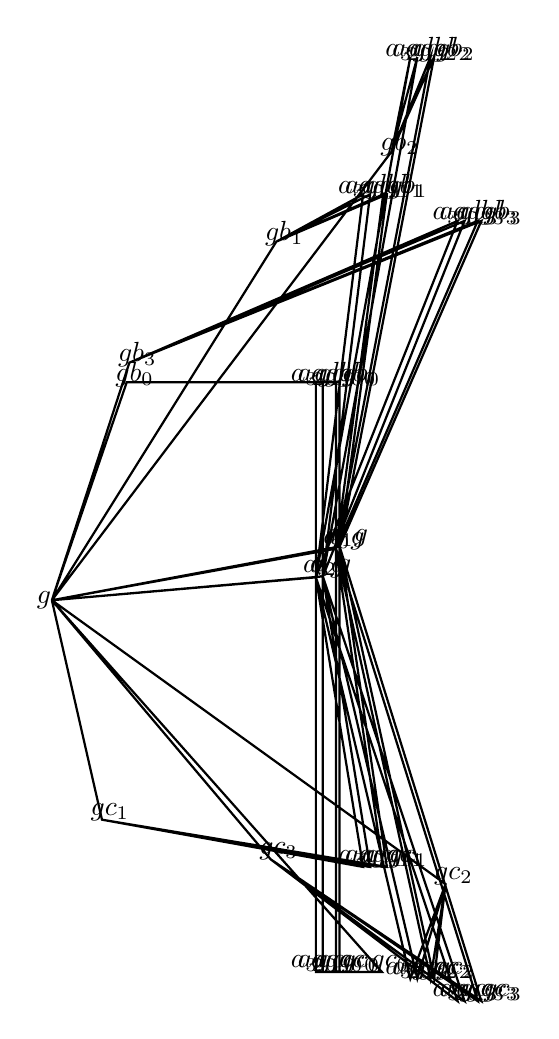
\begin{tikzpicture}
            \draw[thick](0,0)(0,0) -- (0.9509017721415403,2.7683519920800785) -- (3.6084684172201156,2.7683519920800785) -- (3.6084684172201156,0.6555422445425737) -- (0,0)
(0,0) -- (2.8513183788066963,4.5548295332447255) -- (4.208468417220115,5.154829533244725) -- (3.6084684172201156,0.6555422445425737) -- (0,0)
(0,0) -- (4.314832825820895,5.698318288098268) -- (4.808468417220116,6.8983182880982685) -- (3.6084684172201156,0.6555422445425737) -- (0,0)
(0,0) -- (0.9842734385278512,3.0174596536630314) -- (5.408468417220115,4.817459653663031) -- (3.6084684172201156,0.6555422445425737) -- (0,0)
(0,0) -- (0.9509017721415403,2.7683519920800785) -- (3.654136344996517,2.7683519920800785) -- (3.654136344996517,0.6830538810664423) -- (0,0)
(0,0) -- (2.8513183788066963,4.5548295332447255) -- (4.254136344996517,5.154829533244725) -- (3.654136344996517,0.6830538810664423) -- (0,0)
(0,0) -- (4.314832825820895,5.698318288098268) -- (4.854136344996517,6.8983182880982685) -- (3.654136344996517,0.6830538810664423) -- (0,0)
(0,0) -- (0.9842734385278512,3.0174596536630314) -- (5.454136344996517,4.817459653663031) -- (3.654136344996517,0.6830538810664423) -- (0,0)
(0,0) -- (0.9509017721415403,2.7683519920800785) -- (3.441303732553112,2.7683519920800785) -- (3.441303732553112,0.3031778715469337) -- (0,0)
(0,0) -- (2.8513183788066963,4.5548295332447255) -- (4.041303732553112,5.154829533244725) -- (3.441303732553112,0.3031778715469337) -- (0,0)
(0,0) -- (4.314832825820895,5.698318288098268) -- (4.641303732553112,6.8983182880982685) -- (3.441303732553112,0.3031778715469337) -- (0,0)
(0,0) -- (0.9842734385278512,3.0174596536630314) -- (5.241303732553112,4.817459653663031) -- (3.441303732553112,0.3031778715469337) -- (0,0)
(0,0) -- (0.9509017721415403,2.7683519920800785) -- (3.3526965648133062,2.7683519920800785) -- (3.3526965648133062,0.2908128502096852) -- (0,0)
(0,0) -- (2.8513183788066963,4.5548295332447255) -- (3.9526965648133063,5.154829533244725) -- (3.3526965648133062,0.2908128502096852) -- (0,0)
(0,0) -- (4.314832825820895,5.698318288098268) -- (4.552696564813306,6.8983182880982685) -- (3.3526965648133062,0.2908128502096852) -- (0,0)
(0,0) -- (0.9842734385278512,3.0174596536630314) -- (5.152696564813306,4.817459653663031) -- (3.3526965648133062,0.2908128502096852) -- (0,0)
(0,0) -- (4.192400387424257,-4.721799501437912) -- (3.6084684172201156,-4.721799501437912) -- (3.6084684172201156,0.6555422445425737) -- (0,0)
(0,0) -- (0.6364069277259621,-2.786898550881997) -- (4.208468417220115,-3.386898550881997) -- (3.6084684172201156,0.6555422445425737) -- (0,0)
(0,0) -- (4.999832666826254,-3.6052730580674703) -- (4.808468417220116,-4.8052730580674705) -- (3.6084684172201156,0.6555422445425737) -- (0,0)
(0,0) -- (2.7797292674931855,-3.290788200971306) -- (5.408468417220115,-5.090788200971305) -- (3.6084684172201156,0.6555422445425737) -- (0,0)
(0,0) -- (4.192400387424257,-4.721799501437912) -- (3.654136344996517,-4.721799501437912) -- (3.654136344996517,0.6830538810664423) -- (0,0)
(0,0) -- (0.6364069277259621,-2.786898550881997) -- (4.254136344996517,-3.386898550881997) -- (3.654136344996517,0.6830538810664423) -- (0,0)
(0,0) -- (4.999832666826254,-3.6052730580674703) -- (4.854136344996517,-4.8052730580674705) -- (3.654136344996517,0.6830538810664423) -- (0,0)
(0,0) -- (2.7797292674931855,-3.290788200971306) -- (5.454136344996517,-5.090788200971305) -- (3.654136344996517,0.6830538810664423) -- (0,0)
(0,0) -- (4.192400387424257,-4.721799501437912) -- (3.441303732553112,-4.721799501437912) -- (3.441303732553112,0.3031778715469337) -- (0,0)
(0,0) -- (0.6364069277259621,-2.786898550881997) -- (4.041303732553112,-3.386898550881997) -- (3.441303732553112,0.3031778715469337) -- (0,0)
(0,0) -- (4.999832666826254,-3.6052730580674703) -- (4.641303732553112,-4.8052730580674705) -- (3.441303732553112,0.3031778715469337) -- (0,0)
(0,0) -- (2.7797292674931855,-3.290788200971306) -- (5.241303732553112,-5.090788200971305) -- (3.441303732553112,0.3031778715469337) -- (0,0)
(0,0) -- (4.192400387424257,-4.721799501437912) -- (3.3526965648133062,-4.721799501437912) -- (3.3526965648133062,0.2908128502096852) -- (0,0)
(0,0) -- (0.6364069277259621,-2.786898550881997) -- (3.9526965648133063,-3.386898550881997) -- (3.3526965648133062,0.2908128502096852) -- (0,0)
(0,0) -- (4.999832666826254,-3.6052730580674703) -- (4.552696564813306,-4.8052730580674705) -- (3.3526965648133062,0.2908128502096852) -- (0,0)
(0,0) -- (2.7797292674931855,-3.290788200971306) -- (5.152696564813306,-5.090788200971305) -- (3.3526965648133062,0.2908128502096852) -- (0,0)
;
\node at (3.7084684172201157,2.8683519920800786) {$ a_{ 0  } gb_{ 0 } $};
\node at (4.308468417220115,5.254829533244725) {$ a_{ 0  } gb_{ 1 } $};
\node at (4.908468417220115,6.998318288098268) {$ a_{ 0  } gb_{ 2 } $};
\node at (5.508468417220115,4.91745965366303) {$ a_{ 0  } gb_{ 3 } $};
\node at (3.754136344996517,2.8683519920800786) {$ a_{ 1  } gb_{ 0 } $};
\node at (4.354136344996516,5.254829533244725) {$ a_{ 1  } gb_{ 1 } $};
\node at (4.954136344996517,6.998318288098268) {$ a_{ 1  } gb_{ 2 } $};
\node at (5.554136344996516,4.91745965366303) {$ a_{ 1  } gb_{ 3 } $};
\node at (3.541303732553112,2.8683519920800786) {$ a_{ 2  } gb_{ 0 } $};
\node at (4.141303732553111,5.254829533244725) {$ a_{ 2  } gb_{ 1 } $};
\node at (4.741303732553112,6.998318288098268) {$ a_{ 2  } gb_{ 2 } $};
\node at (5.341303732553111,4.91745965366303) {$ a_{ 2  } gb_{ 3 } $};
\node at (3.4526965648133063,2.8683519920800786) {$ a_{ 3  } gb_{ 0 } $};
\node at (4.052696564813306,5.254829533244725) {$ a_{ 3  } gb_{ 1 } $};
\node at (4.652696564813306,6.998318288098268) {$ a_{ 3  } gb_{ 2 } $};
\node at (5.252696564813306,4.91745965366303) {$ a_{ 3  } gb_{ 3 } $};
\node at (3.7084684172201157,-4.621799501437913) {$ a_{ 0  } gc_{ 0 } $};
\node at (4.308468417220115,-3.286898550881997) {$ a_{ 0  } gc_{ 1 } $};
\node at (4.908468417220115,-4.705273058067471) {$ a_{ 0  } gc_{ 2 } $};
\node at (5.508468417220115,-4.990788200971306) {$ a_{ 0  } gc_{ 3 } $};
\node at (3.754136344996517,-4.621799501437913) {$ a_{ 1  } gc_{ 0 } $};
\node at (4.354136344996516,-3.286898550881997) {$ a_{ 1  } gc_{ 1 } $};
\node at (4.954136344996517,-4.705273058067471) {$ a_{ 1  } gc_{ 2 } $};
\node at (5.554136344996516,-4.990788200971306) {$ a_{ 1  } gc_{ 3 } $};
\node at (3.541303732553112,-4.621799501437913) {$ a_{ 2  } gc_{ 0 } $};
\node at (4.141303732553111,-3.286898550881997) {$ a_{ 2  } gc_{ 1 } $};
\node at (4.741303732553112,-4.705273058067471) {$ a_{ 2  } gc_{ 2 } $};
\node at (5.341303732553111,-4.990788200971306) {$ a_{ 2  } gc_{ 3 } $};
\node at (3.4526965648133063,-4.621799501437913) {$ a_{ 3  } gc_{ 0 } $};
\node at (4.052696564813306,-3.286898550881997) {$ a_{ 3  } gc_{ 1 } $};
\node at (4.652696564813306,-4.705273058067471) {$ a_{ 3  } gc_{ 2 } $};
\node at (5.252696564813306,-4.990788200971306) {$ a_{ 3  } gc_{ 3 } $};
\node at (-0.1,0) {$ g $};
\node at (3.7084684172201157,0.7555422445425737) {$ a_{ 0 }g $};
\node at (3.754136344996517,0.7830538810664422) {$ a_{ 1 }g $};
\node at (3.541303732553112,0.40317787154693374) {$ a_{ 2 }g $};
\node at (3.4526965648133063,0.39081285020968526) {$ a_{ 3 }g $};
\node at (1.0509017721415403,2.8683519920800786) {$ gb_{ 0 } $};
\node at (2.9513183788066963,4.654829533244725) {$ gb_{ 1 } $};
\node at (4.414832825820895,5.798318288098268) {$ gb_{ 2 } $};
\node at (1.0842734385278512,3.1174596536630315) {$ gb_{ 3 } $};
\node at (4.292400387424257,-4.621799501437913) {$ gc_{ 0 } $};
\node at (0.7364069277259621,-2.6868985508819967) {$ gc_{ 1 } $};
\node at (5.099832666826254,-3.5052730580674702) {$ gc_{ 2 } $};
\node at (2.8797292674931856,-3.1907882009713058) {$ gc_{ 3 } $};

            \end{tikzpicture}
            \end{center}
            \caption{Square of the complex, with edges $(g,ag), (agb, gb) \in E_A,
            (g,gb), (agb, ag) \in E_B.$ \label{fig:square}
            }
            \end{figure}
 
%\end{multicols*}
  % \printbibliography 
\end{document}

 